%&pdflatex
\documentclass[conference]{IEEEtran}
\usepackage{graphicx}
\usepackage{algorithm2e}
\usepackage{subfigure}
\begin{document}
\title{Forage RRT - An Efficient Approach To Task-Space Goal Planning for Redundant Manipulators}
\author{Leo Keselman\\
	School of ECE\\
	 Georgia Institute of Technology\\
	 L.D.Keselman@gmail.com \and
	Patricio Vela\\ 
	School of ECE\\
	Georgia Institute of Technology\\
	 pvela@ece.gatech.edu
}
\maketitle
\section{Introduction}
One of the ultimate goals of motion planning algorithms for manipulators is to allow the manipulator to automatically find a collision-free
path in a general environment between any given start configuration and a goal point specified in end-effector space coordinates. The goal
is ideally specified in end effector space coordinates because it is almost always the end effector which interacts with the object to be
manipulated. The specific configuration of the other links of the manipulator is usually not important as long as it is not in collision
with workspace obstacles. Examples of end effector tools which interact with objects include hands, magnets, suction cups, paint sprayers,
and welders. Thus, any practical manipulator planner has to convert end-effector space goal coordinates to configuration space goal
coordinates, i.e. the configuration of the manipulator which achieves the given end effector goal coordinate.

In the literature, the two main approaches to solving this problem have been to either figure out the configuration-space goal coordinate
directly using inverse kinematics or to incorporate the search for the configuration space goal coordinate into the planning. To date, we
are not aware of any inverse kinematics algorithm for general n-link manipulators which is complete, fast, and returns a configuration
guaranteed to be reachable from the start configuration. Incorporating inverse kinematics into the planning, especially when the planning
algorithm is the Rapidly-Exploring Random Tree (RRT) alleviates all of these problems. However, this approach struggles to efficiently solve
a certain class of problems, known as bug-trap problems, wherein the approach to the start or goal is largely occluded by an obstacle. If
the configuration of the goal were known, this problem could be satisfactorily solved by the Bidirectional RRT. 

In this paper we present the Forage RRT, which searches for the goal configuration as part of planning but also tackles bug trap type
problems with relative ease. The result is a reliable planner which is fast and consistent at solving a wide range of manipulation problems
in environments with obstacles. The main idea behind the approach is to initially explore the manipulator space quickly with a large
step-size RRT and then attempt to connect to goal using a small step-size Jt-RRT from promising nodes in the large step-size RRT. The Forage
RRT lends itself to parallel implementation and we show that this provides further improvement in average planning times. We believe the
ease of implementing this approach along with its excellent performance on all problems will allow it to be used as a general manipulation
planner both in industry and academia.

The layout of this paper will be to present previous work which we build upon as well as other approaches to the same problem, an analysis
of the shortcomings of the RRT in bug-trap problems, the implementation of the Forage-RRT algorithm, experiments and results compared to
other planners having the same problem statement, and finally a discussion of possible improvement to the Forage RRT.  

\section{Problem Statement}
In this research, we are attempting to develop a motion planner for redundant manipulators which is complete, single-query, and reliably
fast for all reasonable problems posed. The goal of the plan is expected to be specified as an end-effector configuration, either position
only or position and rotation. The only assumptions are that the model of the manipulator is known (at least enough to calculate a
Jacobian) and that the world can be queried to see if a given manipulator configuration would produce a collision or not.

\section{Related Work}
To date, no complete motion planning algorithms are tractible for high dimensional systems such as manipulators. However, over the last 30
years or so, many algorithms have been presented that solve high dimensional motion planning problems. One of the most famous and most cited
approaches is the Artificial Potential Field Method originally presented in \cite{khatib86}. Although this method is fast enough to be
used in a single query planner, it depends on obstacles being of a simple geometry and, as \cite{koren91} points out, suffers from several
fundamental issues such as getting stuck in local minima, no passage between closely spaced obstacles, and oscillations in certain
conditions. Several attempts have been made (e.g. \cite{connolly90} \cite{ge00}) to solve these issues by the formulation of new potential
functions. However, these functions either take prohibitively long to compute or ignore some of the previously mentioned pitfalls. 

\cite{bessiere93} introduced Ariadne's Clew Algorithm which was the first algorithm to approximate C-space by sampling. It was resolution
complete and respectably fast for most problems. Algorithms based on probabilistic roadmaps, deriving from \cite{amato96} used the sampling
idea to pre-process a roadmap for multi-query problems which allowed subsequent path planning problems to be solved efficiently. Because the
preprocessing step takes on the order of minutes, it is not appropriate for our stated goal of a planner for general environments. The
Rapidly-Exploring Random Tree (RRT) was introduced by \cite{lavalle00} as an efficient resolution-complete sampling-based algorithm. In
recent years, this algorithm has been extremely popoular and effective in solving many high dimensional planning problems.

Standard RRTs depend on a start and a goal given in configuration space. This allows for a bidirectional algorithm, also presented in
\cite{lavalle00}, which is effective in solving single bug-trap problems, wherein either the goal or start is largely occluded by an
obstacle, by growing two trees - sometimes randomly, sometimes toward each other. Since goals are most often not specified in configuration
space for manipulation problems, much research has been dedicated to finding inverse kinematics algorithms to transform the goal into
configuration space. Some of the most famous ones are given in \cite{goldenberg85}, \cite{guez88}, \cite{chang87}, \cite{parker89}. None of
these algorithms are complete and guaranteed to be reachable from the start configuration. \cite{ahuactzin99} presented an inverse
kinematics approach that was guaranteed to return a configuration reachable from start. We compare the results of this algorithm to our own
in Section~\ref{sec:evaluation}. 

The other approach to the inverse kinematics problem is to incorporate it into the planning search. This makes the inverse kinematics
complete and guaranteed to be reachable. The first paper to use this approach was \cite{bertram06}, which biased the RRT search to be around
the nodes already added which were closest in end-effector space to goal. Significant speed improvements were achieved by \cite{vande07} in this
approach by using the Jacobian transpose to take steps in the direction of the goal from the existing tree. This approach, however, is very
susceptible to getting stuck when the goal is occluded by an obstacle. Finally, \cite{diankov08} and \cite{yao05}  improved on the idea by
growing an end-effector space tree and using this tree to bias the growth of the configuration-space tree. \cite{diankov08} grew
the end-effector space stree from the goal in a bidirectional type approach whereas \cite{yao05} made end effector paths from start to goal. This
approach too struggles to find solutions quickly in bug-trap problems.
 
\section{RRT and the Bug-Trap Problem}
\label{sec:bugtraprrt}

\begin{figure}[h!]
  \centering
    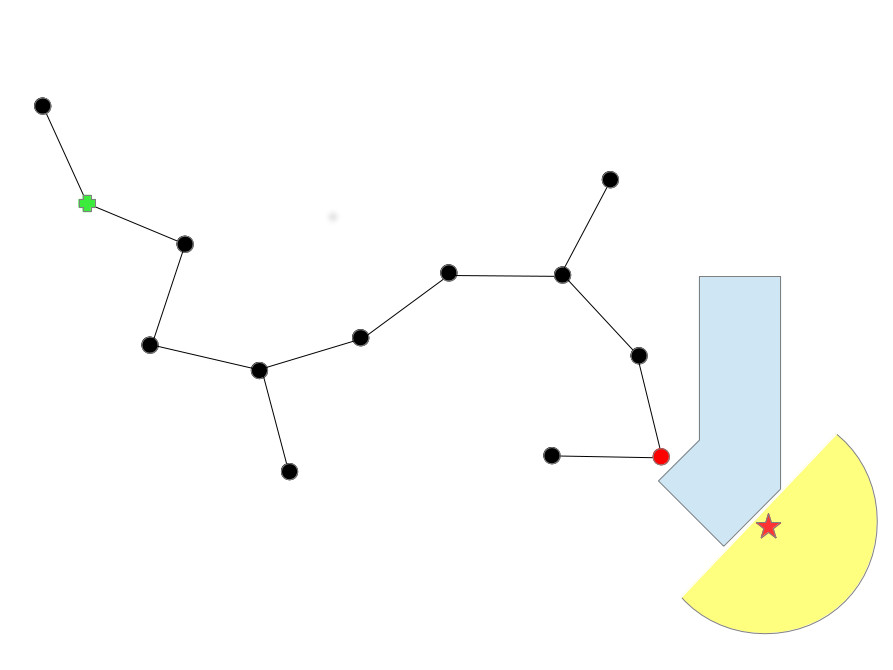
\includegraphics[width=0.5\textwidth]{figures/bugTrapRRT.jpg}
  \caption{An RRT attempting a bug trap problem. \label{fig:BugTrapRRT} }
\end{figure}

Figure~\ref{fig:BugTrapRRT} shows an example of a single style RRT attempting to solve a problem where the goal is occluded by an object.
The state of the RRT is shown after 12 iterations of the extend operation. In this case, the probability of taking a step to goal was
35\%. At this state we can see that two problems emerge in our quest to connect the tree to the goal node:
\begin{enumerate}
\item Future attempts to step to goal will be taken from the red node since it is closest. All these attempts will fail because there is an
obstacle in the way. Obviously, these attempts are a waste of time.
\item To actually get to the goal, the RRT will have to find its way into the yellow semicircle around the goal by virtue of only random
steps. Any nodes outside of this area will be either further than the red node or obstructed by the obstacle. The probability of this
happening quickly is very low. Essentially, it would require that random configurations to extend toward constantly be in the bottom right
corner of the workspace. In this case, the probability of getting such random configurations looks to be around 1/15. In a different
scenario with a larger workspace and smaller step size, this probability would be much smaller. 
\end{enumerate}

Some may argue that this problem occurs because the RRT is too greedy - that if the probability of stepping to goal was smaller, we would be
able to avoid the obstacle. This is not really the case. We can practically throw out the probability that the RRT will reach the goal
randomly, so we still need the tree to extend where a goal step would be useful. This is again a low probaility proposition if the goal is
near the edge of the workspace and occluded by an obstacle. Moreover, less greedy RRTs naturally take longer to converge to goal in simpler
cases. In our opinion, the important takeaway is that fast RRTs generally tend to approach the goal in a very directed fashion.

\section{Forage RRT Implementation}
\label{sec:implementation}
The Forage RRT is based on a similar concept to the Ariadne's Clew Algorithm \cite{bessiere93} in that there are two repeating phases to the
algorithm - explore and search. However, in the Forage RRT, the explore phase is the extension or a coarse step-size RRT and the search phase
is an attempt to connect a node from the coarse step-size tree to the goal via a fine step-size RRT. The relationship to foraging is that
there's a combination of exploring a large space to find leads and the closer investigation of these leads. The effect of this approach for
bug-trap type problems is to solve the problem presented in Section~\ref{sec:bugtraprrt} by using the coarse step-size RRT to find
promising approach directions to the goal and then using the fine step-size RRT to avoid any small occlusions that remain on the path to the
goal.

\subsection{Goal Heap}
One of the inherent inefficiencies in the basic RRT algorithm is that unsuccessful steps to goal may continuously be taken from the same
node because that node is the closest to goal. The problem is illustrated in Section~\ref{sec:bugtraprrt}, Figure~\ref{fig:BugTrapRRT},
where steps to goal from the red node are doomed to fail indefinitely. In RRT implementations for static environments, it is unnecessary and
inefficient to continue to attempt steps to goal from nodes from which such a step has already been attempted - if it did not reach goal
before, it will not again. 

Our solution to the problem is to implement a Goal Heap. When new nodes are added to the tree, they are also added to the goal heap along
with their value. In our case, the value of a node was simply the inverse of its distance to goal. The heap data structure automatically
orders the nodes by value so that the top of the heap is the highest value node. Once a step to goal is attempted from a node, that node is
removed from the Goal Heap because using it again for a step to goal would be a fruitless endeavor.

Although we recommend using a Goal Heap for any RRT implementation to improve efficiency, it is essential for the Forage RRT because it is
used to decide which node in the coarse step-size RRT should be used to attempt a fine step-size RRT to connect to goal.

\subsection{RRT Extend Implementation}
For random extensions of the search tree, we use the standard extension procedure of picking a random point in configuration space and
taking a step towards it from the nearest neighbor already in the tree. For extensions toward the goal, we use the Moore-Penrose
pseudo-inverse Jacobian to take a step in the proper direction. Note that this is similar to the Jt-RRT presented in \cite{vande07} but we
found that using the pseudo-inverse instead of the transpose of the Jacobian was the more effective approach. The overall extend
implementation is shown in Algorithm~\ref{alg:extend}. When implementing this algorithm, one should take good care to make sure that nodes
added to the tree are not only valid configurations themselves but that the link between the new node and its parent is valid. In a fine
step-size RRT this is trivial because we can assume that if the new node is valid, the link too is valid. However, for a coarse step-size
RRT this assumption cannot be made. Instead, the link must be checked by iterating through its length at an acceptable resolution and making
sure each step is also valid.
\begin{algorithm}
 \label{alg:extend}
 \SetAlgoLined
 \KwData{$RRT, goal, StepSize$}
 \KwResult{$Updated RRT, StepResult$}
 \eIf{$randomNumber(0,100) < randomExtendProbability$}{
	$x_{randConfig} \leftarrow RANDOM\_STATE()$\;
	$x_{near} \leftarrow NEAREST\_NEIGHBOR(randConfig, RRT)$\;
	$x_{new} \leftarrow COMPUTE\_NEW\_STATE(x_{randConfig}, x_{near}, stepsize)$\;
	\eIf{$isLegalState(x_{new})$}{
		$RRT \leftarrow addVertex(x_{new})$\;
		$RRT \leftarrow addEdge(x_{near}, x_{new}, StepSize)$\;
		$NodeValue \leftarrow value(x_{new})$\;
		$GoalHeap \leftarrow insert(x_{new}, NodeValue)$\;
		\eIf{$x_{new} = x_{randomConfig}$}{
			$return \; STEP\_REACHED$\;
		}{
			$return \; STEP\_PROGRESS$\;
		}
	}{
		$return \; STEP\_COLLISION$\;
	}	
  }{	
	$x_{near} \leftarrow GoalHeap \rightarrow top$\;
	$x_{new} \leftarrow takeJacobianStep(x_{near}, goal, StepSize)$\;
	\eIf{$isLegalState(x_{new})$}{
		$RRT \leftarrow addVertex(x_{new})$\;
                $RRT \leftarrow addEdge(x_{near}, x_{new}, StepSize)$\;
		\eIf{$x_{new} = goal$}{
                        $return \; GOAL\_REACHED$\;
                }{
			$NodeValue \leftarrow value(x_{new})$\;
	                $GoalHeap \leftarrow insert(x_{new}, NodeValue)$\;
			$GoalHeap \leftarrow remove(x_{near})$\;
                        $return \; STEP\_PROGRESS$\;
                }	
	}{
		$GoalHeap \leftarrow remove(x_{near})$\;
		$return \; STEP\_COLLISION$\;
	}
 }
\caption{RRT Extend Operation}
\end{algorithm}

\subsection{Explore/Search}
The main Forage RRT algorithm is shown in Algorithm~\ref{alg:ForageRRT}. The purpose of the first while loop is to effectively explore the
space and build up several promising nodes to start the fine step-size RRT from. The second while loop attempts to connect the promising
nodes from the coarse step-size RRT to the goal with a fine step-size RRT. Once a fine step-size RRT has endured a certain number of
collisions, we give up on it and try to start another one from the next most promising node. Once a certain number of the fine step-size
RRTs fail, we grow our coarse step-size RRT some more to replenish some promising start nodes. This constant giving up and restarting from
promising nodes allows us to make the fine step-size RRT greedy, making it fast in easy situations but also robust to be able to handle
harder situations. A full list of parameters we used is given in Section~\ref{sec:evaluation}.

Note that once the fine step-size RRT has reached the goal, we can trace back from this node through its parents to the coarse step-size RRT
node that created it and then continue tracing back to the root of the coarse step-size RRT to make our final plan. 

Finally, it is important to note that because of the mixed step size RRTs, the raw final plan will not be attractive, especially near the
start. For this purpose, smoothing is required to make the path acceptable. This is done in a quick manner by taking pairs of nodes,
attempting to connect them with a straight line, and deleting all nodes in between if successful. We have found in this case that the
best way to pick pairs of nodes to attempt to connect is by taking one from the coarse section and the other from the fine section.  The
second step is to go through remaining coarse steps and subdivide them into the desired step size to match the rest of the path.
Empirically, 15-20 pairs of attempted connections makes for a smooth path. 

\begin{algorithm}
 \label{alg:ForageRRT}
 \SetAlgoLined
 \KwData{start, goal}
 \KwResult{path from start to goal}
	$CoarseRRT \leftarrow INITIALIZE(largeStepSize, start, goal)$\;
	\While{$CoarseRRT \rightarrow size < initialSize$}{
		$CoarseRRT \rightarrow EXTEND()$\;
	}
	\While{$result \neq GOAL\_REACHED$}{
		$FineRRT \leftarrow INITIALIZE(fineStepSize, CoarseRRT \rightarrow GoalHeap \rightarrow top)$\;
		\While{$numCollisions < maxNumCollisions$}{
			$FineRRT \rightarrow EXTEND()$\;
		}
		increment numFailures \;
		\If{numFailures = maxNumFailures}{
			\For{1:percentIncrease*initialSize}{
				$CoarseRRT \rightarrow EXTEND()$\;
			}
		}
	}
\caption{Forage RRT}
\end{algorithm}

\subsection{Parallel Implementation}
The separate nature of the Forage RRT search and explore functions make it an ideal candidate for parallel implementation. We used a
Master-Worker approach to the parallel implementation which is described here:
\begin{itemize}
\item \textbf{Initial Step: } Grow coarse step-sze RRT to an initial size greater than the number of threads to be used.
\item \textbf{Worker Threads: } Attempt to connect fine step-size RRT to goal when seeded with start configuration from coarse step-size
RRT. Terminate when a certain number of collisions occurs.
\item \textbf{Master Thread: } 1) Grow coarse step-size RRT 2) Maintain worker threads by seeding them with the best available node from
coarse step-size RRT when they terminate without success.
\end{itemize}

\section{Experiments and Evaluation}
\label{sec:evaluation}
\subsection{Experiments}
\subsubsection{Sequential Implementation}
Experiments were conducted on a Schunk 7 DOF arm with the DART/GRIP simulator, developed by the GOLEMS lab at Georgia Tech, on a 2.27GHz, 8
core machine. We compared the following algorithms to the smoothed Forage RRT:
\begin{enumerate}
	\item Jt-RRT \cite{vande07}
	\item Moore-Penrose Pseudo-Inverse RRT: this is the same as Jt-RRT aside from using an Moore-Penrose pseudo-inverse Jacobian to take
	      goal directed steps
	\item BiSpace RRT \cite{diankov08}
	\item Kinematic Roadmap \cite{ahuactzin99}: note that the paths produced from this algorithm would be too long to be used for most
	      applications but rather only the inverse kinematics, which is guaranteed to be reachable from start would be used.
\end{enumerate}

It is worth noting that smoothing time was included in Forage RRT results but no other results because the paths produced did not strictly
require it for those cases. Moreover, each RRT was restarted after 10,000 nodes to reduce average planning time of all planners.

Each algorithm was tested on an easy, medium, and hard case, shown in in Figure~\ref{fig:cases} In each figure, the goal is the point where
the three shown faces of the yellow and blue cube meet. 50 random collision-free start configurations were computed for each case (easy,
medium, and hard) and the same 50 start configurations were used for each algorithm. Each start configuration was the seed for 40 runs, thus
totaling 2000 runs per algorithm per case. In the interest of time, a run was considered a failure if the RRT had to be restarted 25 times
and no solution was found. At that point, the run would have taken 400-600 seconds so each failure should be considered a strong penalty. 

\begin{figure*}[t]
  \label{fig:cases}
  \centering
    \subfigure[Easy case for testing: no obstacles. \label{fig:EasyCase}]
     	{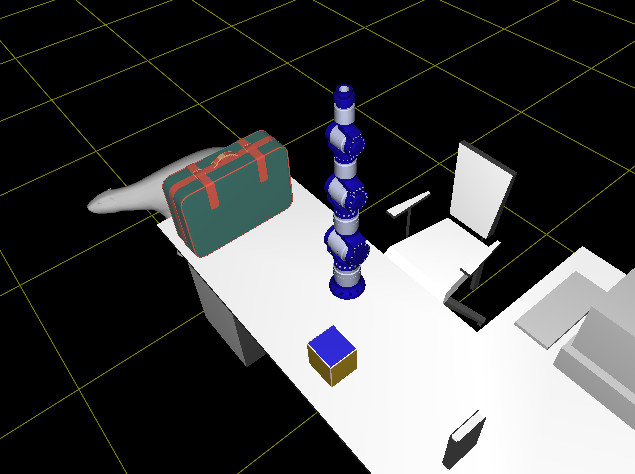
\includegraphics[width=0.29\textwidth]{figures/EasyCase.jpg}}
    \subfigure[Medium case for testing: obstacles throughout space. \label{fig:MediumCase}]
        {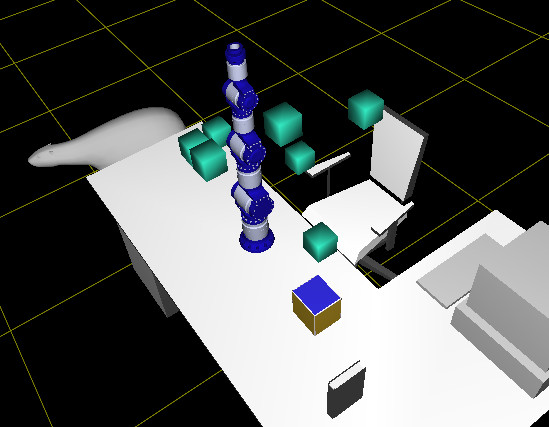
\includegraphics[width=0.29\textwidth]{figures/MediumCase.jpg}}
    \subfigure[Hard case for testing: goal directly under obstacle, near edge of workspace. \label{fig:HardCase} ]
    	{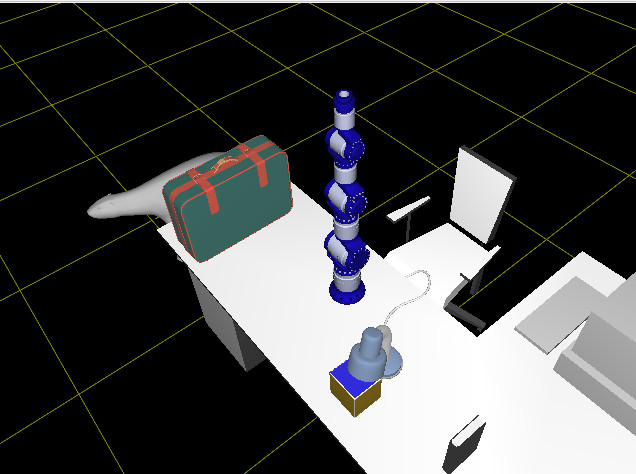
\includegraphics[width=0.29\textwidth]{figures/HardCase.jpg}}
    \caption{Depiction of different test cases.}
\end{figure*}

The Forage RRT parameters used for testing are given in Table~\ref{tab:ForageParams}

\begin{table}
	\centering
	\begin{tabular}{| c | c | }
        	\hline
		initialSize & 50 \\ \hline
  		randomExtendProbability - coarse & 90 \\ \hline
  		randomExtendProbability - fine & 65 \\ \hline
  		largeStepSize & 1.3\\ \hline
  		fineStepSize & .02\\ \hline
  		maxNumCollisions & 5\\ \hline
  		maxNumFailures & 10\\ \hline
		percentIncrease & .25\\ \hline 
	\end{tabular}
	\caption{Forage RRT parameters.} 
	\label{tab:ForageParams}
\end{table}

\subsubsection{Parallel Implementation}
To understand the properties of the parallel algorithm, experiments were conducted on the same cases as the sequential Forage RRT. The
parallel implementations were tested for 10 precomputed start configurations per case, at 40 runs per start configuration. Thus, each
version was tested 400 times. The implementation was tested with 1,2,3,4,5, and 6 worker threads. The results were simulated using the
DART/GRIP simulator and run on a 2.27GHz, 8 core machine.

\subsection{Evaluation}
For the purpose of visualization, an example of the end effector positions of the coarse RRT are shown in in Figure~\ref{fig:CoarseRRT}.
It's evident to see that the closest nodes to goal come from many different directions, making the fine RRTs more likely to be effective.
The green node is the start and the red node is the goal.

\begin{figure}[h!]
  \centering
    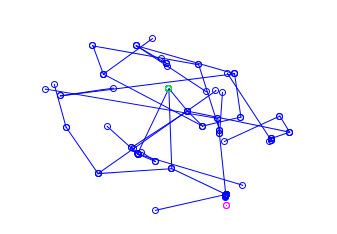
\includegraphics[width=0.5\textwidth]{figures/coarseRRTExample.jpg}
  \caption{End effector positions for the initial coarse RRT. \label{fig:CoarseRRT} }
\end{figure}


\subsubsection{Sequential Implementation}
The results of the sequential implementation simulation are shown in Table~\ref{tab:Results}. The reported times are averaged over completed
cases only. Failures are runs that took 400-600 seconds and did not find a solution so should be taken as a strong negative penalty to the
algorithm.

\begin{table*}
        \centering
        \begin{tabular}{| c | c | c | c | c | c | c | }
		\hline
                Algorithm & \textbf{Easy Avg} & \textbf{\% Comp} &\textbf{Med Avg} & \textbf{\% Comp} & \textbf{Hard Avg} & \textbf{\% Comp}\\  \hline
                \textbf{Forage RRT}&\textbf{2.92}&\textbf{100}&\textbf{3.01}&\textbf{100}&\textbf{7.52}&\textbf{100}\\ \hline
                \textbf{Jt-RRT}&12.12&93.7& & &62.62&29.0\\ \hline
                \textbf{Jinv-RRT}&4.45&96.9&21.42&92.0&65.92&53.6\\ \hline
		\textbf{BiSpace RRT}&4.57&100&21.94&99.96&36.87&80.6\\ \hline
   		\textbf{Kin. Roadmap}&5.22&100& & &22.24&100\\ \hline
        \end{tabular}
        \caption{Sequential experiment results. All times in seconds.}
        \label{tab:Results}
\end{table*}

\subsubsection{Parallel Implementation}
The results of the parallel implementation are shown for different numbers of extra worker threads in Figure~\ref{fig:ParallelResults}. The
results show a decline in average planning time when using the parallel implementation. The decline is not linear but neither should we
expect it to be. Because the solution is often found in the first few attempts to connect to goal from the coarse RRT, extra threads working
on other start points are not going to be helpful. A decline in performance is seen with 5 and 6 worker threads. We suspect this is because
the threads start interfering with each other. Even though the machine we used for testing has 8 cores, some of them are used partially for
other processes running on the machine. In any case, the results that improvements after 4 working threads would be minimal. The best
average planning times achieved with the parallel implementation are summarized in Table~\ref{tab:BestParallel} and apply to the case when 4
worker threads were implemented.

\begin{figure}[h!]
  \centering
    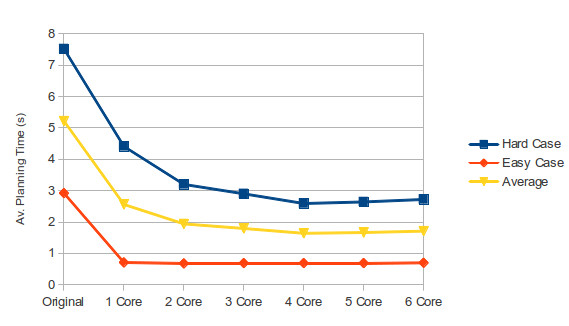
\includegraphics[width=0.5\textwidth]{figures/ParallelResults.jpg}
  \caption{Average planning times per number of extra cores used. \label{fig:ParallelResults} }
\end{figure}

\begin{table}
        \centering
        \begin{tabular}{| c | c | }
                \hline
                Case & \textbf{Av. Planning Time} \\  \hline
                Easy & .69 \\  \hline
		Medium & \\  \hline
		Hard & 2.59 \\  \hline
		Average &\textbf{} \\  \hline
        \end{tabular}
        \caption{Parallel (4 core) results. All times in seconds.}
        \label{tab:Results}
\end{table}



\section{Discussion}
\subsection{Completeness}
As shown in \cite{lavalle00}, any RRT is complete because its coverage of the workspace converges to the sampling distribution. Because the
coarse RRT in the Forage RRT algorithm searches indefinitely, the Forage RRT is also complete. Needless to say, it is highly unlikely in
practice that the coarse RRT will be the one to come upon the goal.

\subsection{Parameters}
The Forage RRT parameters used to achieve the results in Table~\ref{tab:Results} are given in Table~\ref{tab:ForageParams}. These parameters
were arrived at empirically and by no means are guaranteed to be ideal ones. It may be of interest to investigate ideal values for these
parameters, for instance when to switch from fine searching to coarse searching. In theory, it could be based on some function instead of a
hard number of failures. Moreover, parameters such as initial coarse tree size and coarse tree step size may be good candidates for learning
over time. It is quite possible that the ideal values for these parameters depend on specific environment factors such as the volume of the
workspace. The Forage RRT algorithm presented in Section~\ref{sec:implementation} should be a very strong base line for any motion planning
environment, especially one for a manipulator, but improvements could foreseeably be made to make it more adaptible to any environment.

\subsection{Replanning}
In situations where the environment has changed but the start and goal have not, the Forage RRT lends itself to possible future work in
replanning strategies. For instance, it may be faster to modify the parts of the coarse tree affected by the environment changes than to
rebuild the whole tree. Another idea may be to reuse the coarse node which was a successful start for the fine RRT in the previous run as a
waypoint in the search to bias the tree toward an area which is likely to be successful again.

\section{Conclusion}
We have presented the Forage RRT algorithm for motion planning. We believe the algorithm's efficieny on tough problems, consistency,
completeness, ease of implementation, and parallel potetial make it the best available motion planning algorithm for general
problems where the goal is specified in task space. We have shown its effectiveness specifically for redundant manipulators.

\bibliographystyle{plain}
\bibliography{RRT,MotionPlanning,IK}

\end{document}

